\documentclass[../masters.tex]{subfiles}

\begin{document}
\graphicspath{{./imgs/}{../imgs/}} %look for images

\section{Nonlinear Models}
In this section we consider probabilistic graphical models of the form shown in Figure \ref{fig_linmod}. This model is a generalisation of the graphical model seen in the Hidden Markov Model section. We now assume that the states ($X = x_1,x_2,...$) and observations ($Y=y_1,y_2,...$) are continuous random variables but the inputs ($U=u_1,u_2,...$) are deterministic. Models of this form are called Latent Linear Dynamical Systems (the famous Kalman Filter model falls into this category).
\begin{figure}[H] 
\centering
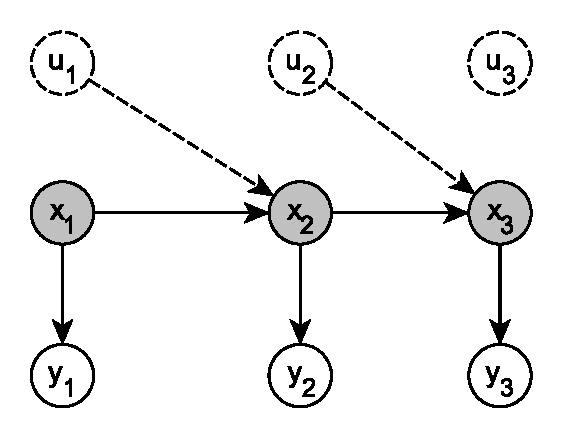
\includegraphics[scale=1.0]{linear_model.pdf}
\caption{Graphical model of this section}
\label{fig_linmod}
\end{figure}
In the previous section we developed inference algorithms but assumed that the transition and observation functions were discrete. We also noted that this assumption is not appropriate for continuous data. The reason is that one would invariably need to discretise the domain of the continuous random variable under consideration. This would result in intractably large discrete systems if one requires fine resolution. To address this issue we extend the previous model to include both continuous states and observations. 

We assume linearity and that all the random variables are Gaussian. While these are strong assumptions they form the building blocks of much more expressive models as we will discover in the next section. We also assume that the transition and emission functions are time invariant. The state space model is of the form (\ref{eq_statespace}).
\begin{equation}
\begin{aligned}
x_{t+1} &= Ax_t + Bu_t + w_{t+1} \text{ with } \mathcal{N}(w_{t+1}|0,Q) \\
y_{t+1} &= Cx_{t+1} + v_{t+1}  \text{ with } \mathcal{N}(v_{t+1}|0,R)
\end{aligned}
\label{eq_statespace}
\end{equation}
Rewriting the state space model we see that the transition and emission functions are given by (\ref{eq_trans_emiss}). Note that we also assume that the system is first order Markov.
\begin{equation}
\begin{aligned}
p(x_{t+1}|x_t, u_t)&= \mathcal{N}(x_{t+1}|Ax_t+Bu_t, Q) \\
p(y_{t+1}|x_t) &= \mathcal{N}(y_{t+1}|Cx_{t+1}, R)
\end{aligned}
\label{eq_trans_emiss}
\end{equation}
We have implicitly assumed that the noise is Gaussian and white\footnote{The noise is temporally independent, has zero mean and finite variance.}. Intuitively one can think of $R$ being the covariance of the noise associated with state measurements and $Q$ being the uncertainty (plant-model mismatch) associated with the linear model of the plant. Additionally, $Q$ can also model any unmeasured disturbances which may influence the system\footnote{Note that for the purposes of this dissertation plant is a synonym for the system.}. Thus, larger $R$ and $Q$ indicate more uncertainty in the system. 

To fully specify the system we require the transition and emission functions (these implicitly depend on the internal structure of the graphical model in Figure \ref{fig_linmod}) as well as the prior (initial) distribution of $x_1$.



\subsection{Filtering the CSTR}

\subsection{Controlling the CSTR}

\bibliographystyle{plain}
\bibliography{research}

\end{document}